
The grid construction is called by the \textit{Grid Factory} (see \ref{interface-grid-factory}) after all the vertices, elements and boundary segments have been inserted. The construction of the \curvgrid{} is in accordance with the following plan

\begin{mybox}
\begin{enumerate}
	\item Construction of grid entities - Interior ($I$), Process Boundary ($PB$), Domain Boundary ($DB$) and Interior Boundary ($IB$) edges and faces.
	\item Construction of the global index for all entities. By default, the global index for vertices and elements is re-used from the mesh file.
	\item Construction of Ghost elements ($G$)
	\item Construction of entity subsets used for iteration over different entity partition types and codimensions
	\item Construction of communication maps, used to perform communication via the \textit{DataHandle} interface
	%\item Construction of OCTree for hierarchical element location
\end{enumerate}
\end{mybox}


\subsection{Storage}
\label{impl-grid-storage}

\noindent
The paradigm used in \curvgrid{} is to store all data corresponding to the grid in a single class, namely the \textit{CurvilinearGridStorage} class. Entities of each codimension are stored in arrays indexed by the local entity index, which is contiguous and starts from 0 on all processes. Each entity stores its global index, geometry type and partition type. For the detailed explanation on the correct assignment of partition types to entities of each codimension, the user is referred to the corresponding section of \dune{} grid usage manual, found on the website of the project. Elements and faces also store the associated material (physical) tag. Elements store the local index of all interpolatory vertices in the \textit{Sorted Cartesian} order (see \cref{impl-gmsh-numbering-convention}). The edges and faces do not store the interpolatory vertex indices, as it would be wasteful for higher curvilinear orders. Instead, each edge and face is stored as a subentity of an associated parent element - any of the elements containing it. Thus, each subentity stores the parent element local index, as well as the subentity index, by which the subentity is indexed within the reference element. Finally, each face stores its boundary type - Interior, Domain Boundary or Periodic Boundary, as well as the index of the 2nd parent element that shares it. By convention, the primary parent element must always be interior to the process storing the face. The secondary parent element may be either interior, or Ghost (\cref{fig:impl:ghostelements}). The data associated with a Ghost element is stored on the neighboring process, but can be accessed from this process as part of interprocessor communication. In case of Domain Boundaries, there is no secondary parent. By convention, any attempts to access the secondary parent of a Domain Boundary result in an exception, as the user code must take the provided partition type into account when addressing neighboring entities. \\

\noindent
\curvgrid{} contains several different local index sets, designed to uniquely index only the entities of a given subset. Namely, Domain Boundary segments, Interior Boundary segments, Process Boundaries, remaining Interior boundaries, as well as Ghost elements each have their own local index. \curvgrid{} provides maps between those indices and local indices of all entities of a given codimension. In addition, there is a unique index for grid corners, namely the interpolatory vertices that define the linear entities (\cref{fig:impl:storage:vertexvscorner}). This is necessary, because the \dune{} facade class operates in terms of linear elements, and thus requires a contiguous index for the corners. Importantly, among all vertices only entity corners possess unique process boundary index, since, for all interprocessor communication purposes, the mesh can be assumed to be linear without loss of generality. Finally, a map from global to local index is provided for entities of all codimensions. \\

\begin{figure}
    \centering
	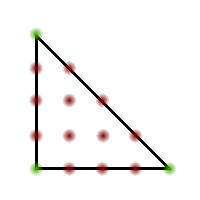
\includegraphics[scale=1.5]{images/vertex-vs-corner}
	\caption{The interpolatory vertices of the 5th order curvilinear triangle. Corners are given in red}
	\label{fig:impl:storage:vertexvscorner}
\end{figure}

\noindent
\curvgrid{} operates with two different types of \textit{GlobalIds}, designed to uniquely identify the entity among all processes. First of all, it is a pre-requisite that all vertices have an associated global index, which is either re-used from the mesh file, or constructed in the beginning of the grid construction procedure. Before the global indices for other codimensions are generated, these entities are uniquely identified by the sorted set of global indices of the entity corners, which can be used in a map to determine if a given communicated entity is already present on the receiving process. Later, when entities of all codimensions possess global index, the \textit{GlobalId} is simply a wrapper of the global index, such as to use minimal amount of resources necessary. It is the latter \textit{GlobalId} that is made available for the user code at the end of construction procedure. \\

\noindent
For the purposes of iterating over frequently used entity subsets, the corresponding local index subsets are provided for each codimension. Namely, subsets are provided for all entities of a given codimension, Interior entities, Process Boundary entities, Domain Boundary entities, Ghost entities, Interior + Domain Boundaries (called \textit{interior} in \dune{}), Interior + Domain Boundaries + Process Boundaries (called \textit{interior border} in \dune{}). \\

\noindent
For communication purposes, all communicating entities need to store a vector of ranks of processes with which these entities are shared. For more details on communicating entities, see \cref{impl-grid-constructor-comm}.




\subsection{Global index construction}
\label{impl-grid-constructor-globalindex}

\noindent
In this section we briefly describe the algorithm used to construct the global indices for all codimensions. The challenge in computing the global indices comes from the fact that originally the processes are not aware of their neighbors. Due to the insertion of complete boundary segments by the grid factory, each process can readily identify all of its process boundaries as the faces that have only one containing element on the process and are not already marked as domain boundaries. The algorithm has four definite stages - determining the neighboring process for each process boundary, assigning (virtual) ownership of each shared entity to only one of the processes sharing it, enumerating the global index on processes owning the entities, and communicating the global index to all other processes containing each shared entity. \\

\noindent
The algorithm starts by determining neighbor ranks of each Process Boundary ($PB$) corner. Currently, each process communicates all process boundary corner global indices to all other processes. From the received global indices each process can deduce all other processes sharing each of its corners. Then, each process assigns provisional neighbor processes to edges and faces by considering the processes that share all entity corners. If two processes share all the corners of a given entity, it does not mean that they share the entity as well (\cref{fig:impl:globalindex:fakeedge}). The ambiguity is quite rare, because most entities are shared only by two processes, and since each process boundary entity must be shared by at least two processes, there is no need to check if the entity exists. Nevertheless, the grid must be able to handle the rare case of an entity being shared by more than two processes. In this case, the edge and face \textit{GlobalIds} (see \cref{impl-grid-storage}) are communicated to all provisional neighboring processes. Each of the provisional neighbor processes then responds, whether or not each entity corner set corresponds to an entity. The ranks that are not confirmed to share the entities are then removed from the neighbor list. \\

\begin{figure}
    \centering
	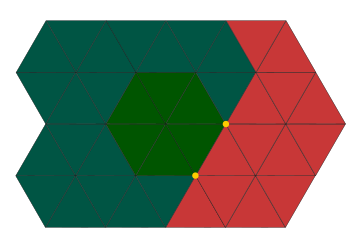
\includegraphics[scale=0.5]{images/parallel-fake-edge}
	\captionsetup{width = 0.8\textwidth}
	\caption{The two yellow vertices are shared between three processes. The edge in-between them only exists on red and green processes, but not on the blue one}
	\label{fig:impl:globalindex:fakeedge}
\end{figure}

\noindent
For each $PB$ edge and face, an owner is determined. The ownership strategy is flexible, as long as all processes agree. Currently, a shared entity is considered to be owned the process with the lowest rank among those sharing it. Each process owns all of its non-shared entities. The number of entities owned by each process is then communicated to all other processes. \\

\noindent
Each process then locally enumerates the global index of all its entities. To begin with, each process computes the shift in global index due to the entities of each codimension enumerated by the processes with ranks lower than this process rank. All processes enumerate global indices consecutively, starting with 0 on rank 0 process. This constructs a global index individually for each codimension. A global index over all entities is also constructed, shifting the enumeration also by all the enumerated entities of higher codimension. \\

\noindent
The enumerated global indices are then communicated among all processes sharing the entities. By analyzing entity neighbors, each process can compute how many global indices it needs to send to and receive from each other process, avoiding extra communication. At the end of this process, the global-to-local index map is filled on each process.



\subsection{Ghost element construction}
\label{impl-grid-constructor-ghost}

\noindent
Ghost entities are the subentities of the element on the other side of the process boundary face, including the element itself. The process boundary entities are not considered Ghost entities. Thus, the Ghost entities are the internal/domain boundary entities of another process, borrowed by this process. Construction of Ghost entities involves communicating all the information associated with the entities to the neighboring processes, and then incorporating the Ghost entities into the grid on the receiving side (\cref{fig:impl:ghostelements}). \\

\begin{figure}
    \centering
	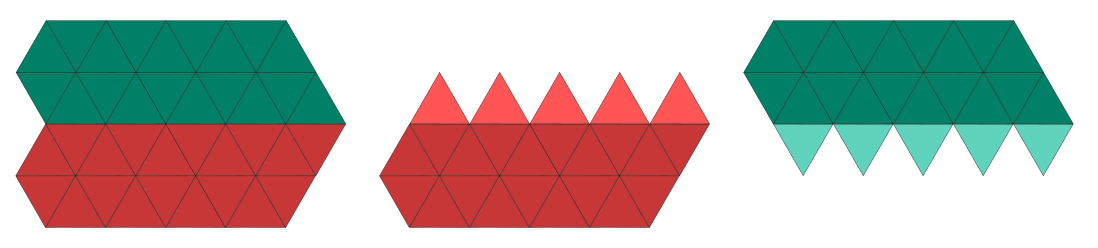
\includegraphics[scale=0.5]{images/parallel-ghost-elements}
	\caption{The first image depicts two neighboring processes without Ghost elements. The second and third images contain only the first and only the second process entities respectively, including Ghost elements borrowed from the other process. }
	\label{fig:impl:ghostelements}
\end{figure}

\noindent
Since for every $PB$ face the neighboring process rank has already been determined in the previous section, and the global index is already known, it remains only to communicate the corresponding neighbor entities and correctly integrate them into the local grid. Firstly, one needs to communicate the properties of the structure to be communicated. Thus, for each interior element next to the $PB$ the interpolation order is communicated, as well as the number of $PB$ faces it shares with the receiving side. It is important to note that a Ghost element can have more than one $PB$ face associated to it, and the receiving side does not know in advance that two or three of its $PB$ faces are associated with the same Ghost element. This is also the reason it is not possible to know in advance how many ghosts will be received from a neighbor process. Afterwards, for each Ghost element the global index, physical tag, global indices of all codimension subentities and subentity indices of $PB$ faces of the element are communicated. The corresponding Ghost elements are then added to the mesh, and it is determined which vertex coordinates are missing. The vertex coordinates are not communicated immediately, because the neighbor process may already have some of the global coordinates due to narrow mesh appendices. Thus, each process communicates the number of vertex coordinates missing from each of its neighbors, and then communicates the missing coordinates.




\subsection{Communication interface construction}
\label{impl-grid-constructor-comm}

The communication paradigm of \dune{} \textit{DataHandle} interface is to communicate data between instances of the same entity on different processes. Depending on the communication protocol, only entities of specific structural types will communicate. We will slightly redefine the partition type classes in this section for compactness reasons. There are three different communicating partition types
\begin{itemize}
	\item $PB$ - Process boundary entities, that is, process boundary faces and their subentities
	\item $I$ - Interior entities, including the $DB$ but excluding the $PB$ entities.
	\item $G$ - Ghost elements and their subentities, excluding $PB$
\end{itemize}


\begin{figure}
    \centering
	\begin{subfigure}[b]{0.48\textwidth}
	  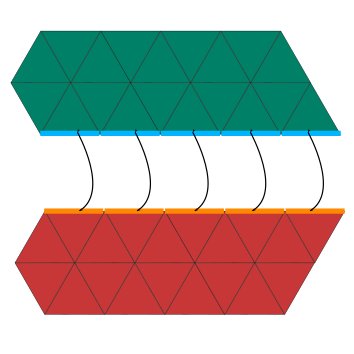
\includegraphics[scale=0.4]{images/parallel-comm-PBPB}
	  \captionsetup{width=0.8\textwidth} 
	  \caption{$PB \leftrightarrow PB$. Communication of neighboring process boundaries}
	\end{subfigure}
	\begin{subfigure}[b]{0.48\textwidth}
	  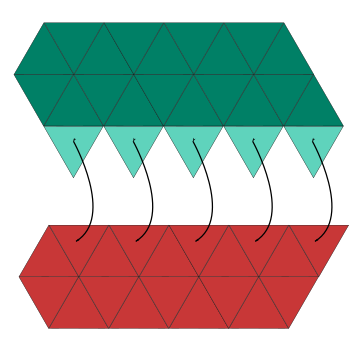
\includegraphics[scale=0.4]{images/parallel-comm-IG}
	  \captionsetup{width=0.8\textwidth} 
	  \caption{$I \leftrightarrow G$. Communication of interior element and its Ghost on another process }
	\end{subfigure}
	\begin{subfigure}[b]{0.48\textwidth}
	  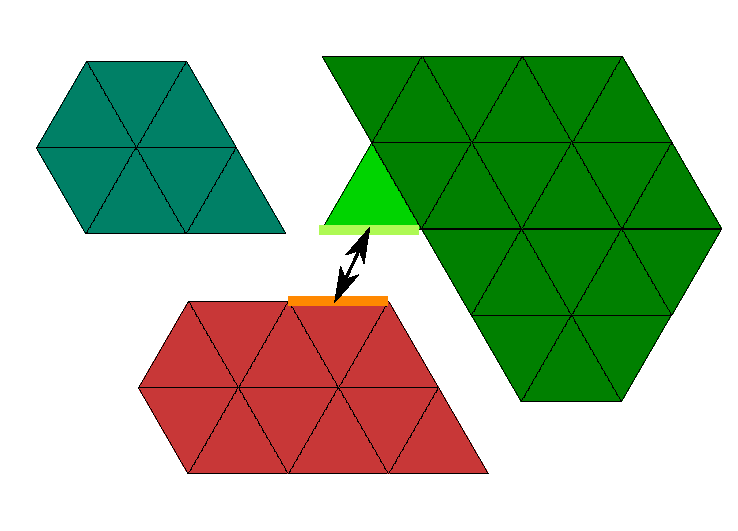
\includegraphics[scale=0.4]{images/parallel-comm-PBG}
	  \captionsetup{width=0.8\textwidth} 
	  \caption{$PB \leftrightarrow G$. Communication of a Ghost of the blue process on the green process with a process boundary on the red process}
	\end{subfigure}
	\begin{subfigure}[b]{0.48\textwidth}
	  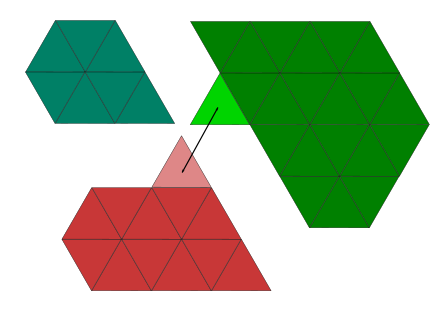
\includegraphics[scale=0.4]{images/parallel-comm-GG}
	  \captionsetup{width=0.8\textwidth} 
	  \caption{$G \leftrightarrow G$. Communication between two ghosts of the same element of the blue process on the green and the red process}
	\end{subfigure}
	\captionsetup{width=0.8\textwidth}
	\caption{ Partition type pairs that can communicate to each other}
	\label{fig:impl:comm:partitionpairs}
\end{figure}


\noindent
We consider all partition type pairs, for which the \textit{DataHandle} communication is possible (\cref{fig:impl:comm:partitionpairs}). Note that interior entities only communicate to Ghost and vice-versa, because Process Boundaries are Process Boundaries on both neighboring processes. However, Process Boundaries can communicate to Ghosts and vice-versa, because a process boundary can be a Ghost with respect to a third process at the triple point. \\

\noindent
The \textit{DataHandle} interface foresees four communication protocols. The \cref{table:impl:datahandle:protocols} presents the communication interfaces used by Dune, and explains how they translate to communication between entities of above specified partition types \\

\begin{table}
\centering
\begin{tabular}{ | l | l | l | l | l | l | l | l | }
  \hline
  Interface & Direction &
      \small $PB \rightarrow PB$ \normalsize &
      \small $PB \rightarrow G$ \normalsize &
      \small $I \rightarrow G$ \normalsize &
      \small $G \rightarrow I$ \normalsize &
      \small $G \rightarrow PB$ \normalsize &
      \small $G \rightarrow G$ \normalsize \\ \hline 
  \begin{tabular}[x]{@{}c@{}}\lstinline|InteriorBorder_|\\ \lstinline|InteriorBorder| \end{tabular}
  & ---      & Y & N & N & N & N & N \\ \hline
  \lstinline|InteriorBorder_All|            & Forward  & Y & Y & Y & N & N & N \\ \hline
  \lstinline|InteriorBorder_All|            & Backward & Y & N & N & Y & Y & N \\ \hline
  \lstinline|All_All|                       & ---      & Y & Y & Y & Y & Y & Y \\ \hline
\end{tabular}
\caption{Communication interfaces of \textit{DataHandle}, and the associated communicating partition type pairs}
\label{table:impl:datahandle:protocols}
\end{table}


\noindent
The aim of this part of the grid constructor is to generate/reuse unique index maps for the sets $PB$, $I$ and $G$. Then, for every communicating entity, for every possible partition type pair, we require an array of ranks of the processes for which such communication is possible. Note that the map for the pair $PB\rightarrow PB$ already exists, it is constructed in the very beginning of the grid construction procedure to enable global indices and Ghost elements. The algorithm is as follows:

\begin{mybox}
\begin{enumerate}
	\item Mark the neighbor process ranks of the associated $PB$ for all $I$ and $G$ entities, whose containing elements neighbor $PB$, thus enabling the $I \rightarrow G$ and $G \rightarrow I$ communication. Note that entities of all (!!) codimensions can have more than one neighbor rank obtained this way. During the marking, elements with two or more process boundaries from different processes may be encountered. In that case, for each process boundary entity the rank of the other process boundary is marked, thus providing some information for the future construction of the $PB \rightarrow G$ communications.
	\item Then, all entities that can communicate are associated with ranks of all other processes, over which the entities are shared.% It remains to finish the $PB \rightarrow G$ communication, and calculate the remaining protocols $G \rightarrow I$, $G \rightarrow PB$ and $G \rightarrow G$.
	\item For all $PB$ entities, subtract $PB\rightarrow PB$ set from the $PB \rightarrow G$ set to ensure that the latter excludes the former. Also, mark the number of effective $PB \rightarrow G$ candidate entities of each codimension for each process
	\item For all $PB$ entities with non-empty $PB \rightarrow G$ set, communicate $G$ indices to all neighboring $PB$ entities
	\item For all $PB$, append the union of the received $G$ to the $PB \rightarrow G$ set, thus completing it %(hopefully)
	\item For all $PB$ entities with non-zero $PB \rightarrow G$, communicate self index to all $G$ of $PB \rightarrow G$ set
	\item For all $G$, append the union of the received $PB$ to the $G \rightarrow PB$ set, thus completing it %(hopefully)
	\item For all $PB$ entities with non-zero $PB \rightarrow G$, communicate to all own $G$ neighbors all the other $G$ in the set
		%\subitem Optimization - do this only if you are lowest rank among all $PB$-neighbors
		%\subitem Further optimization - do this only if you are modulus-rank among all $PB$-neighbors
	\item For all $G$, append the union of the received $G$ to the $G \rightarrow G$ set, thus completing it %(hopefully)	
\end{enumerate}
\end{mybox}



    


% 
% \subsection{Iteration set construction}
% \label{impl-grid-constructor-iterator}
% 
% Construction of the iterator sets involves simply iterating over all entities, and filling the sets with local indices based on the entity structural type.
% 
% 
% \subsection{OCTree construction}
% \label{impl-grid-constructor-octree}





